\documentclass[conf]{new-aiaa}
%\documentclass[journal]{new-aiaa} for journal papers
\usepackage[utf8]{inputenc}
\usepackage{import}
\usepackage{hyperref}
\usepackage{graphicx}
\usepackage{amsmath}
\usepackage[version=4]{mhchem}
\usepackage{siunitx}
\usepackage{longtable,tabularx}
\usepackage{placeins}
\usepackage{transparent}
\usepackage{pdflscape}
\usepackage{afterpage}
\usepackage{tablefootnote}
\setlength\LTleft{0pt}
\usepackage[table,xcdraw]{xcolor}
\usepackage{natbib}
\graphicspath {{figures/}}


\usepackage{subcaption}


\usepackage{subcaption}
\usepackage{booktabs}
\usepackage{float}
\usepackage{multirow}
\usepackage{geometry}
\usepackage{amsfonts}
\usepackage{amssymb}
\usepackage{tikz}

\usetikzlibrary{arrows,chains,positioning,scopes,shapes.geometric,shapes.misc,shadows}


\usepackage{array}
\newcolumntype{L}[1]{>{\raggedright\let\newline\\\arraybackslash\hspace{0pt}}m{#1}}
\newcolumntype{C}[1]{>{\centering\let\newline\\\arraybackslash\hspace{0pt}}m{#1}}
\newcolumntype{R}[1]{>{\raggedleft\let\newline\\\arraybackslash\hspace{0pt}}m{#1}}


\setlength\LTleft{0pt}

\title{EECS 587 Project: Parallel-in-time algorithms for system sensitivities}
\author{Josh Anibal}
% \author{Charles A. Mader\footnote{Research Investigator, AIAA Senior Member}}
% \affil{University of Michigan, Ann Arbor, Michigan}

\begin{document}

\maketitle


% Notes
% - unsteady problems are of interest
%    - active flow control
%    - acoustics

% time averaged objective function





% unroll coupled loops?



% \section{Nomenclature}

% {\renewcommand\arraystretch{1.0}
% \noindent\begin{longtable*}{@{}l @{\quad=\quad} l@{}}
% $A$  & amplitude of oscillation \\
% \end{longtable*}}




\begin{abstract}

    Gradient-based-optimization is ideal for engineering design optimization problems, which typically have a large number of design variables.
    However, gradient-based-optimizers require sensitivity information to drive the objective function to a minimum.
    Even if analytical methods are used, sensitivity routines can be a bottleneck for large engineering models or when coupled analyses are used.


    % This is similar to backward propagation for neural networks except a linear system may need to be solved for each step making some steps more expensive and the process must be repeated for each objective and constraint.

    % Because there are typically more design variables than functions of interest, model sensitivities are calculated in the reverse mode.
    In forward mode differentiation, the inputs of one analysis's sensitivity routine are provided by the outputs of sensitivity routines earlier in the execution order.
    The same is true for reverse mode differentiation, but the execution order of the sensitivity routines is the opposite of the model execution order.
    Because each sensitivity routine only depends on results of prior routines, there is a time-like dependency structure between sensitivity routines.

    Parallelizing tasks with a time-like dependency structure is non-trivial, but will become increasingly important to achieve good performance as computer architectures become increasingly concurrent.
    It is for this reason we propose using algorithms developed for parallel-in-time execution to parallelize the computation of sensitivities for engineering models.
    In this work we will highlight any gains in performance from the execution of parallel-in-time sensitivity analysis for a low-fidelity heat-transfer constrained design problem. % or an aerostructural problem?
    We will do this by implementing our engineering model and sensitivity analysis inside the open source optimization framework OpenMDAO \cite{Gray2019a}.



\end{abstract}





\section{Introduction}


% engineering models are complicated
Engineering models are composed of many sub-analyses.
For example, in aerospace engineering a model to predict the fuelburn of an aircraft may be composed of analyses to compute geometry, aerodynamic performance, structural stresses, engine performance, and trajectory.
Each of those analyses may be coupled with an other and many consist of many more sub-analyses.

- optimization frameworks make it easy for users to construct large models
- show openaeostruct n2 diagram to show scale of system


% optimization uses models
To use a model, such as the fuelburn model, in large scale design optimization one needs to write sensitivity routines for each analysis.
For an analysis that solves PDEs this may involve using the adjoint or the direct method.
Then to calculate the gradients needed by the optimizer the sensitivity routines can be used in the forward or reverse mode.
% either way the sensitivity routines have time dependency struture
In the forward mode the each sensitivity routine is only influenced by those that came before in the model execution order and in the reverse mode each routine is only affected by those that come after.
In either sensitivity mode, the dependency of the routines is one way.

% this structure is common
This one-way dependency structure is very similar to that of a time-accurate simulation where each time step is only influenced by those that came before it.
Because this type of simulation is so common, research effort has already been applied to parallelize these simulations in time despite the difficulty inherent to the dependency structure.

from wiki
"While historically most efforts to parallelize the numerical solution of partial differential equations focussed on the spatial discretization, in view of the challenges from exascale computing, parallel methods for temporal discretization have been identified as a possible way to increase concurrency in numerical software.[2]"

% work has been done on this problem
Gander\cite{Gander2015} provides a review of this work and showcases key contributions.
The author of the review highlights the recent increased interest in parallel-in-time algorithms now that processor clock speeds have plateaued.
The current trend in computing is toward using increased parallelism to provide increased performance.
This trend is unlikely to reverse anytime soon especially as GPUs find there way into mainstream computing.

% poeople are applying this work else where
Because of the rising importance of parallelism, recent work has been done to apply the research on algorithms for parallel time accurate simulations to problems with the same structure.
Gunther et al.\cite{Gunther2019} have shown that the parallel-in-time algorithm MGIRT\cite{Falgout2014} was effective at reducing the computational time required to solve for sensitivities of an unsteady adjoint problem.
Furthermore, Gunther et al.\cite{Gunther2020} have applied the same technique to speedup backpropogation for neural networks and shown its effectiveness.


% this hasn't be applied to general engineering models yet
At present no work has been done to parallelize the execution of sequential sensitivity routines within the sensitivity computation for engineering models.
The aim of this work is to address this absence by applying parallel-in-time algorithms to this task and highlighting the performance enhancements.


\section{Problem}
To explore the idea of using PinT algorithms to speed up sensitivity calculations we first need a problem to test our algorithm on.

Since this study is exploratory a suitable problem should be rather basic.
However, it must also be scalable so that we may fully test the algorithm.

To stratify these requirements our model will consist of N identical components connected in series.
In this model each component only passes values to the component ahead of it and only recieves values from the component behined it.
Similarly when calculating sensitivities in the reverse mode, the derivative seeds are propogated backwards from the last component to the first.

-- figure of components passing values forward and derivatives back --


Although, this problem represents a vary simple dependency structure between components it incorporates the key difficult in computing sensitivities; passing information all the way from one side of the model to the other.


Within each component a linear system will have to be solved to calculated the derivative seeds of the inputs.
This represents a cause where the components cacluate their outputs by solving and implicit equation, which is often the case for models based on PDEs.

It is important that the system that is being solved by each componentne has the same same structure as a real problem.
This is becuase it has been shown that PinT algorithms can have a different effectiveness for matrices which represent different physical problems.

As a result the matrix was carefully chosen.

The matrix was take from a component constructed to solve a steady aeroelastic analysis\cite{Jasa2018a}.
The component uses a vortex lattice method to calculate loads at points along the wing and a beam model to calculate the subsequent deflections
By chaining this component together it represents a model similar to a quasi steady aeroelastic analysis.
The matrix represent the jacobian of the state variables of the system with respect to the residuals.
By varying the finest of the discretization we can create matrices of varying size.
Using this method 417x417, 2387x237, 21830x21830, 90711x90711, 342711x342711 matrices were created.




\section{Algorithm}

The algorithm used to parallelize the sensitivity calculation is based on the parareal algorithm.
Parareal is one of teh most popular PinT algorithms and has a wide body of literacy describing its implementation and performance properties.

% describe what the parareal algorithm is

% decompose the time
The time domain must be decomposed into as many sum domains as the number of processors.
For our sensitivity propogation problem, the domain is the collection of all the models components.
Thus the sub domain are fromed by creating subsets of the the model components


--- sub compontents shown graphically ---


Each processor will work towards solve the problem on its sub domain.
This is done by preforming iterations using a "coarse" and a "fine" methods for solving the problems on the sub domains.
As the names suggest the coarse method should supply an approximate solution to the problem at low cost, while the fine method should supply an arcuate answer to the problem at a much higher cost.

For our sensitivity propogation problem. the fine method will be an accurate solve of the linear system of each component while the coarse method is and inexact solve of the same system.
For both methods the iterative solver GMRES will be used but with different tolerances.
The fine solver has a tolerance of 1e9, which is the smallest tolerance that could be reliably solved, while the coarse method has a tolerance of 1e-5.







The algorithm is initalized by computing a coarse solution to the problem by using sequentially using the coarse solution method on each sub domain.

\begin{equation}
    y_{j+1}=\mathcal{G}\left(y_{j}, t_{j}, t_{j+1}\right), \quad j=0, \ldots, P-1
\end{equation}


Then in parallel each processor computes the solution of the fine problem based on an initial condition of the sub domain using the coarse solution
\begin{equation}
    y_{j+1}=\mathcal{F}\left(y_{j}, t_{j}, t_{j+1}\right), \quad j=0, \ldots, P-1
\end{equation}


A sequential correction is then made based on the fine solution and the difference in coarse solution at current and prior iteration.


\begin{equation}
    y_{j+1}^{k+1}=\mathcal{G}\left(y_{j}^{k+1}, t_{j}, t_{j+1}\right)+\mathcal{F}\left(y_{j}^{k}, t_{j}, t_{j+1}\right)-\mathcal{G}\left(y_{j}^{k}, t_{j}, t_{j+1}\right), \quad j=0, \ldots, P-1, \quad k=0, \ldots, K-1
\end{equation}

Parallel fine solutions and sequential corrections are performed iteratively until the the solution across the entire time domain converges.

"
Because Parareal computes the numerical solution for multiple time steps in parallel, it is categorized as a parallel across the steps method.[3] This is in contrast to approaches using parallelism across the method like parallel Runge-Kutta or extrapolation methods, where independent stages can be computed in parallel or parallel across the system methods like waveform relaxation.[4][5]
"


It can be shown that the parareal algorithm will converge to the exact solution in the general case in P iterations or less.
However, if the algorithm converges in P iterations no speed up will be achieved.
Thus to achieve meaningful speedups with the basic algorithm it must converge in far fewer than P iterations.



To further improve on the basic algorithm, the prior solution can be used as an initial guess for the fine method and the prior coarse solution can be used as an initial guess for the coarse method.
It is import not to use the current solution as the intial guess for the coarse method as this was found to cause the algorithm to converge to the incorrect answer.
This technique requires additional memory to save the prior solution, but reduces the cost next iteration.

Another modification made to the ordinal parareal algorithm was to skip fine solutions and corrections on sub domains which have already converged to the exact solution.
Because the sub domain j, 0< j < P  will converge to the exact solution after J iterations there is no need to update it in future iterations.


This two optimizations reduce the cost of later iterations and lead to a faster algorithm overall.



\subsubsection{Parallelsim}
This algorithm can be parallelized using either shared memory or distributed memory.

For this project MPI was used to incorporate distributed memory parallelism.
Distributed memory parallelism was chosen because the solution methods used on each sub domain may require solving large systems that require lots of memory.
As a result the algorithm may need to be run on multiple nodes.
MPI and distributed memory parallleism provides a flexible solution for supporting inter and intra node parallelization.


messages are pasted backwards during each sequential solve.
blocking communication is used to prevent the processor from moving forward until it has the information it needs to do so.

no barriers are used to allow greater overlap in computation.
Figure ?? shows the ideal case of parallel execution. it was found that load balancing was necessary to achieve this.


--- execution threads in parallel ---




\subsubsection{Load balancing}
It was found that equally distributing the components of the model across processors was not ideal.
For our particular problem it was discovered that components that that were closer to the end took more time to solve both fine and coarse problems.

This was a major issue because during the sequential upate all processor downstream need to wait until the prior has completed it's sequential update.

To ensure the processor were not holding up later processors, the earlier processors were given less work.



Although, it is had to solve this issue in general.
One could use the condition number or eigenvalues of the matrix to estimate how difficult it will be to solve the system.
However, these are expensive to compute and in this example even though all of the components use the same matrix the time to solve still differed by a factor of up to 8.

\section{Results}
algorithm was run on greatlakes

\subsection{strong scaling}
peaks at 1.5x speed up at two procs

performance is poor

\subsection{weak scaling}

also bad

\section{Discussion}

Parallelization in time is inherently difficult.

parareal algorithm speed up is bounded by


\begin{equation}
    S_{p}=\frac{c_{\text {fine }}}{c_{\text {parareal }}}=\frac{1}{(K+1) \frac{N_{c}}{N_{f}} \frac{\tau_{c}}{\tau_{f}}+\frac{K}{P}} \leq \min \left\{\frac{N_{f} \tau_{f}}{N_{c} \tau_{c}}, \frac{P}{K}\right\}
\end{equation}

with plan parareal we need a K << P and a coarse method which is much faster than the fine method to achieve a speedup

\begin{figure}[H]
	\centering
	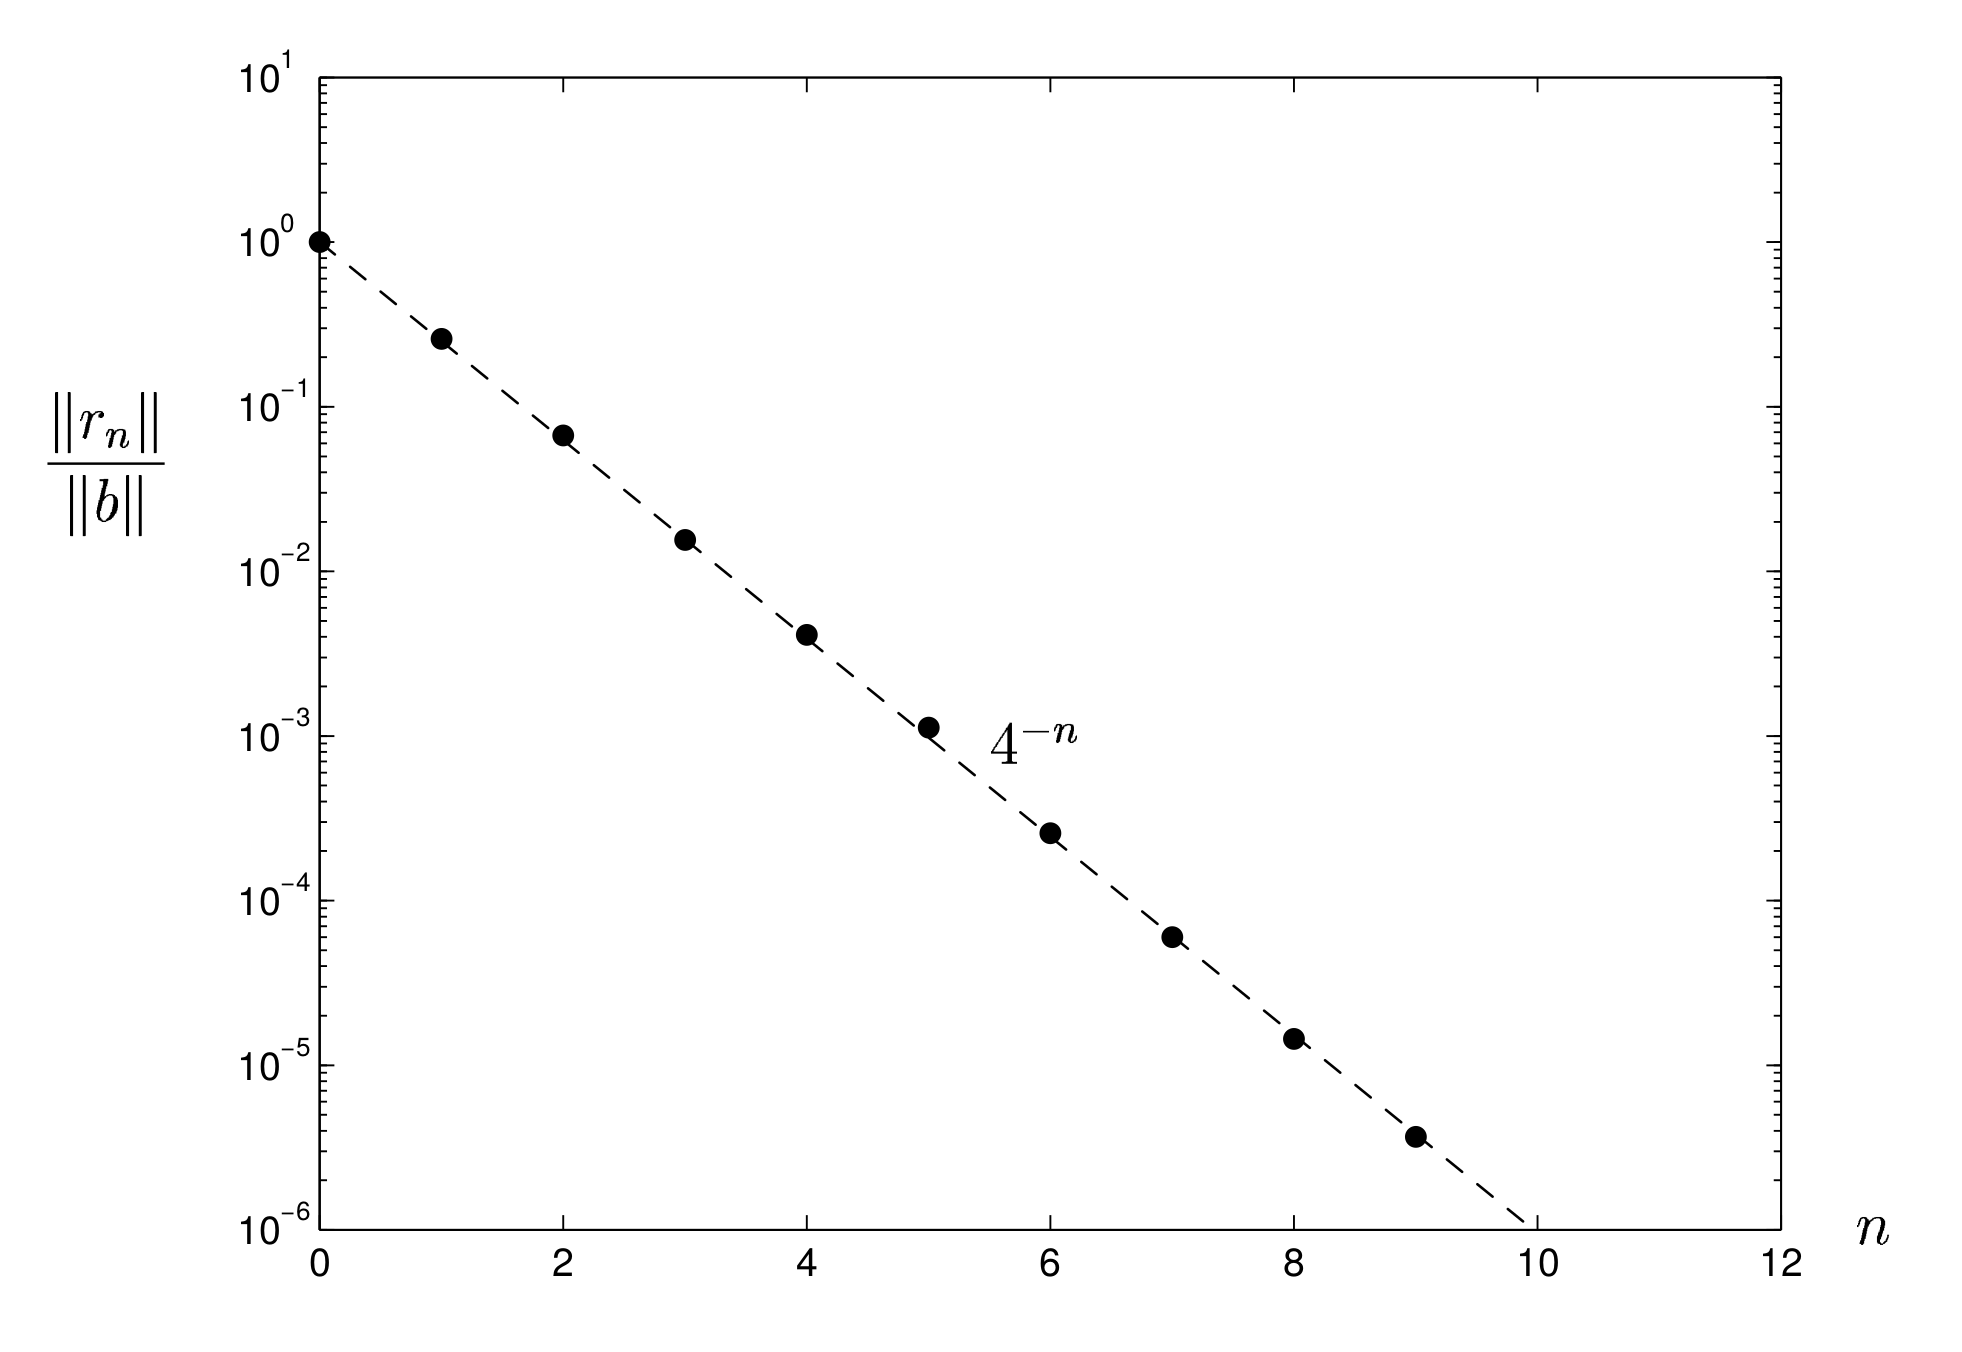
\includegraphics[width=0.60\textwidth,keepaspectratio]{gmres_conv.png}
	\caption{Convergence rate of GMRES for a well behaved matrix from "Numerical Linear Algebra" by Trefethen and Bau}
	\label{fig:gmres_conv}
\end{figure}
gmres converges linearly. This limits the ratio of the costs of the fine and coarse method

\begin{figure}[H]
	\centering
	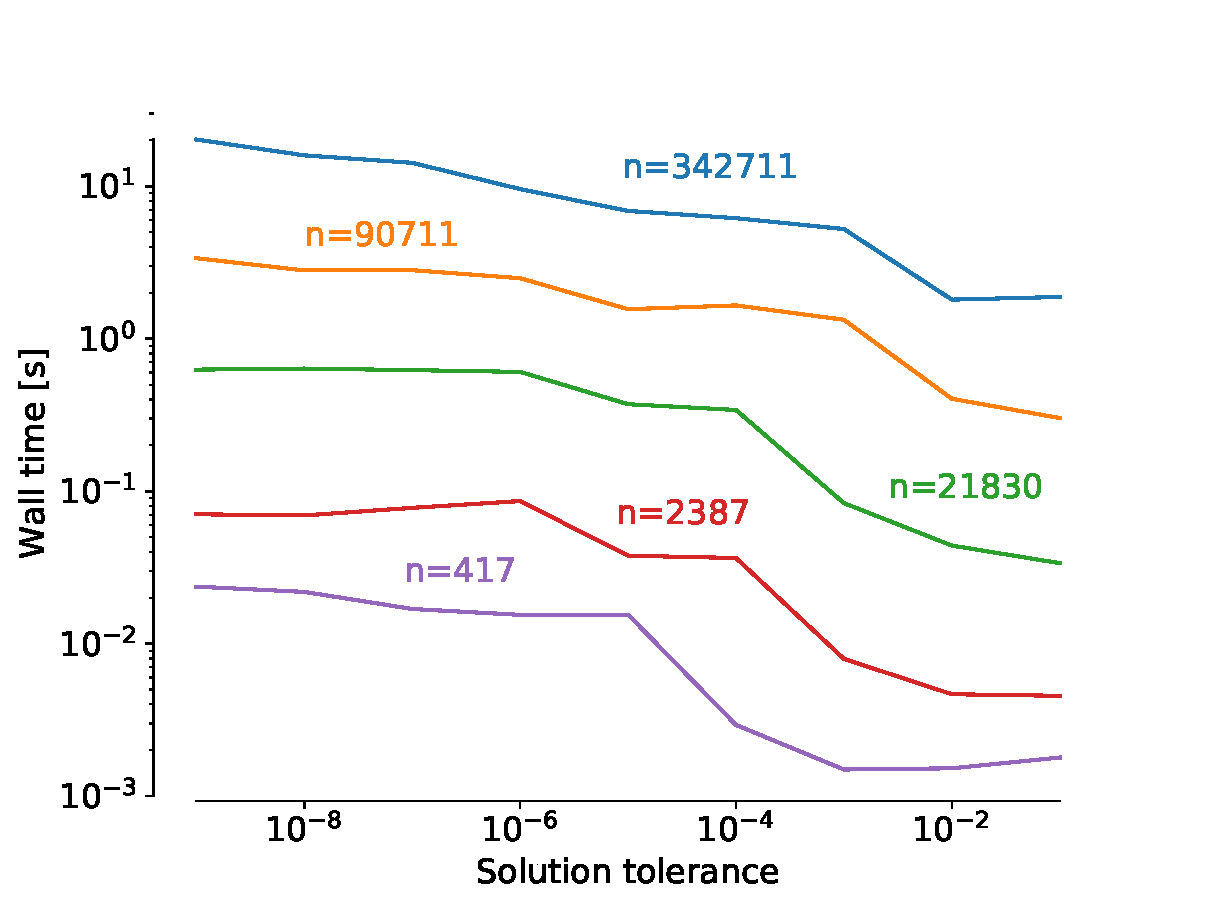
\includegraphics[width=0.60\textwidth,keepaspectratio]{acc_timing.pdf}
	\caption{The cost to solve each matrix using GMRES for a given level of accuracy}
	\label{fig:acc_timing}
\end{figure}



- more or less linear. For twice as many orders of accuracy the cost of the solution only doubles.

Pretty remarkable, but it means that a pure parareal algorithm the max speedup is at most 2x for the levels of fine and coarse solvers used.

the second term $\frac{P}{K}$
-parallel garunetted to converge after P iterations, but then there is no speedup
- arrcurcy of parareal converges like so with K
- high tolerance for coarse solver needed for K to converge sooner than P
- balance with first term

- for our problems it was found that we were unable to converge K in less than P iterations


- by reusing information we can make the cost of additional iterations cheaper, but with only small tweaks we can't do much better than the original parareal algorithm which has no speed up for this problem.

- more effective to just speed up each fine solver.
- using a toolbox like petsc has better scalability up to many many core.
- only really has value has a second layer of parallelism
- one would have to have a massive problem for it to be worth using this algorithm

- or many simple problems which don't parallelize well (like a NN)

\section{conclusion}

don't do this


\bibliography{mybib,mdolab}

\end{document}
